% GNUPLOT: LaTeX picture with Postscript
\begingroup
  \makeatletter
  \providecommand\color[2][]{%
    \GenericError{(gnuplot) \space\space\space\@spaces}{%
      Package color not loaded in conjunction with
      terminal option `colourtext'%
    }{See the gnuplot documentation for explanation.%
    }{Either use 'blacktext' in gnuplot or load the package
      color.sty in LaTeX.}%
    \renewcommand\color[2][]{}%
  }%
  \providecommand\includegraphics[2][]{%
    \GenericError{(gnuplot) \space\space\space\@spaces}{%
      Package graphicx or graphics not loaded%
    }{See the gnuplot documentation for explanation.%
    }{The gnuplot epslatex terminal needs graphicx.sty or graphics.sty.}%
    \renewcommand\includegraphics[2][]{}%
  }%
  \providecommand\rotatebox[2]{#2}%
  \@ifundefined{ifGPcolor}{%
    \newif\ifGPcolor
    \GPcolorfalse
  }{}%
  \@ifundefined{ifGPblacktext}{%
    \newif\ifGPblacktext
    \GPblacktexttrue
  }{}%
  % define a \g@addto@macro without @ in the name:
  \let\gplgaddtomacro\g@addto@macro
  % define empty templates for all commands taking text:
  \gdef\gplfronttext{}%
  \gdef\gplfronttext{}%
  \makeatother
  \ifGPblacktext
    % no textcolor at all
    \def\colorrgb#1{}%
    \def\colorgray#1{}%
  \else
    % gray or color?
    \ifGPcolor
      \def\colorrgb#1{\color[rgb]{#1}}%
      \def\colorgray#1{\color[gray]{#1}}%
      \expandafter\def\csname LTw\endcsname{\color{white}}%
      \expandafter\def\csname LTb\endcsname{\color{black}}%
      \expandafter\def\csname LTa\endcsname{\color{black}}%
      \expandafter\def\csname LT0\endcsname{\color[rgb]{1,0,0}}%
      \expandafter\def\csname LT1\endcsname{\color[rgb]{0,1,0}}%
      \expandafter\def\csname LT2\endcsname{\color[rgb]{0,0,1}}%
      \expandafter\def\csname LT3\endcsname{\color[rgb]{1,0,1}}%
      \expandafter\def\csname LT4\endcsname{\color[rgb]{0,1,1}}%
      \expandafter\def\csname LT5\endcsname{\color[rgb]{1,1,0}}%
      \expandafter\def\csname LT6\endcsname{\color[rgb]{0,0,0}}%
      \expandafter\def\csname LT7\endcsname{\color[rgb]{1,0.3,0}}%
      \expandafter\def\csname LT8\endcsname{\color[rgb]{0.5,0.5,0.5}}%
    \else
      % gray
      \def\colorrgb#1{\color{black}}%
      \def\colorgray#1{\color[gray]{#1}}%
      \expandafter\def\csname LTw\endcsname{\color{white}}%
      \expandafter\def\csname LTb\endcsname{\color{black}}%
      \expandafter\def\csname LTa\endcsname{\color{black}}%
      \expandafter\def\csname LT0\endcsname{\color{black}}%
      \expandafter\def\csname LT1\endcsname{\color{black}}%
      \expandafter\def\csname LT2\endcsname{\color{black}}%
      \expandafter\def\csname LT3\endcsname{\color{black}}%
      \expandafter\def\csname LT4\endcsname{\color{black}}%
      \expandafter\def\csname LT5\endcsname{\color{black}}%
      \expandafter\def\csname LT6\endcsname{\color{black}}%
      \expandafter\def\csname LT7\endcsname{\color{black}}%
      \expandafter\def\csname LT8\endcsname{\color{black}}%
    \fi
  \fi
    \setlength{\unitlength}{0.0500bp}%
    \ifx\gptboxheight\undefined%
      \newlength{\gptboxheight}%
      \newlength{\gptboxwidth}%
      \newsavebox{\gptboxtext}%
    \fi%
    \setlength{\fboxrule}{0.5pt}%
    \setlength{\fboxsep}{1pt}%
\begin{picture}(5000.00,4000.00)%
    \gplgaddtomacro\gplfronttext{%
      \put(1078,0){\makebox(0,0){\strut{}$-\pi$}}%
      \colorrgb{0.15,0.15,0.15}%
      \put(1959,0){\makebox(0,0){\strut{}$-\dfrac{\pi}{2}$}}%
      \colorrgb{0.15,0.15,0.15}%
      \put(2841,0){\makebox(0,0){\strut{}$0$}}%
      \colorrgb{0.15,0.15,0.15}%
      \put(3722,0){\makebox(0,0){\strut{}$+\dfrac{\pi}{2}$}}%
      \colorrgb{0.15,0.15,0.15}%
      \put(4603,0){\makebox(0,0){\strut{}$+\pi$}}%
      \colorrgb{0.15,0.15,0.15}%
      \put(946,264){\makebox(0,0)[r]{\strut{}$10^{-4}$}}%
      \colorrgb{0.15,0.15,0.15}%
      \put(946,743){\makebox(0,0)[r]{\strut{}$10^{-3}$}}%
      \colorrgb{0.15,0.15,0.15}%
      \put(946,1222){\makebox(0,0)[r]{\strut{}$10^{-2}$}}%
      \colorrgb{0.15,0.15,0.15}%
      \put(946,1701){\makebox(0,0)[r]{\strut{}$10^{-1}$}}%
      \colorrgb{0.15,0.15,0.15}%
      \put(946,2181){\makebox(0,0)[r]{\strut{}$10^{0}$}}%
      \colorrgb{0.15,0.15,0.15}%
      \put(946,2660){\makebox(0,0)[r]{\strut{}$10^{1}$}}%
      \colorrgb{0.15,0.15,0.15}%
      \put(946,3139){\makebox(0,0)[r]{\strut{}$10^{2}$}}%
      \colorrgb{0.15,0.15,0.15}%
      \put(1078,3359){\makebox(0,0){\strut{}$-\pi$}}%
      \colorrgb{0.15,0.15,0.15}%
      \put(1959,3359){\makebox(0,0){\strut{}$-\dfrac{\pi}{2}$}}%
      \colorrgb{0.15,0.15,0.15}%
      \put(2841,3359){\makebox(0,0){\strut{}$0$}}%
      \colorrgb{0.15,0.15,0.15}%
      \put(3722,3359){\makebox(0,0){\strut{}$+\dfrac{\pi}{2}$}}%
      \colorrgb{0.15,0.15,0.15}%
      \put(4603,3359){\makebox(0,0){\strut{}$+\pi$}}%
    }%
    \gplgaddtomacro\gplfronttext{%
      \colorrgb{0.15,0.15,0.15}%
      \put(176,1701){\rotatebox{90}{\makebox(0,0){\strut{}$N_s |\delta|$ [m]}}}%
      \colorrgb{0.00,0.00,0.00}%
      \put(2840,3889){\makebox(0,0){\strut{}Επίλοιπο σφάλμα $\phi$: εξ. (\ref{eq:phi2})}}%
      \colorrgb{0.15,0.15,0.15}%
      \put(2840,-400){\makebox(0,0){\strut{}$\phi$ [rad]}}%
    }%
    \put(0,0){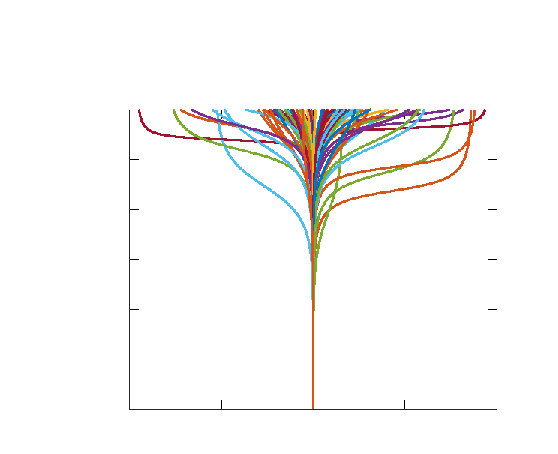
\includegraphics{./figures/parts/02/chapters/04/sections/02/phi_rc_x1}}%
    \gplfronttext
  \end{picture}%
\endgroup
